\subsection{Ejercicio 1}
\graphicspath{ {img/01} }

\subsubsection{Generación claves RSA Cryptool}

\begin{figure}[H]
    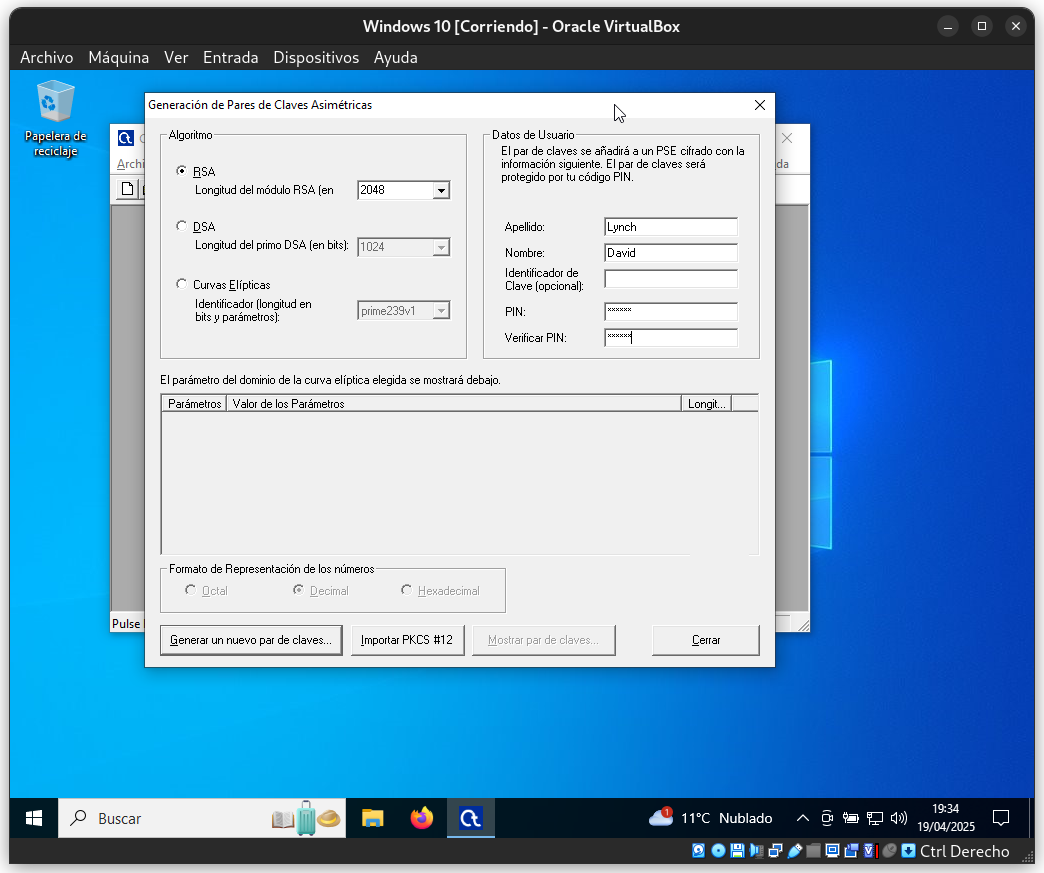
\includegraphics[width=\textwidth]{ClavesRSA-01.png}
    \caption{Generación del perfil del par de claves RSA}
\end{figure}

\begin{figure}[H]
    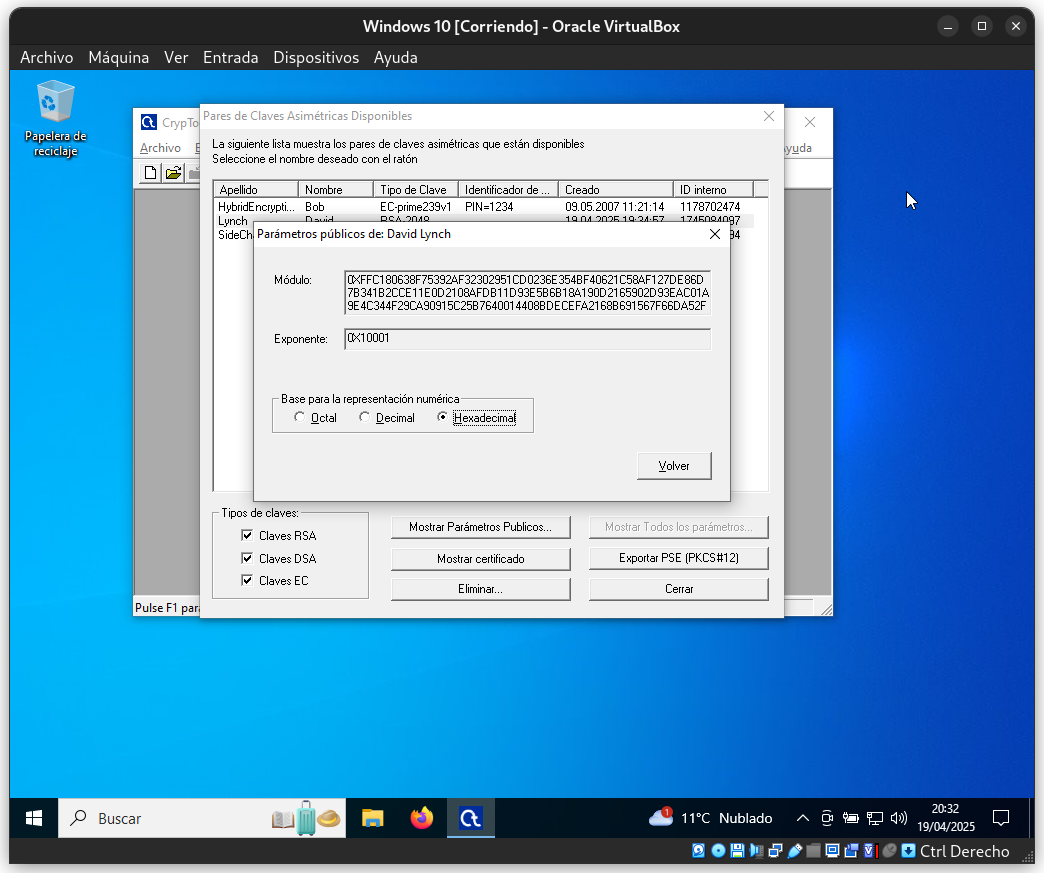
\includegraphics[width=\textwidth]{ClavesRSA-02.png}
    \caption{Parámetros públicos de la clave (n, e)}
\end{figure}

\begin{figure}[H]
    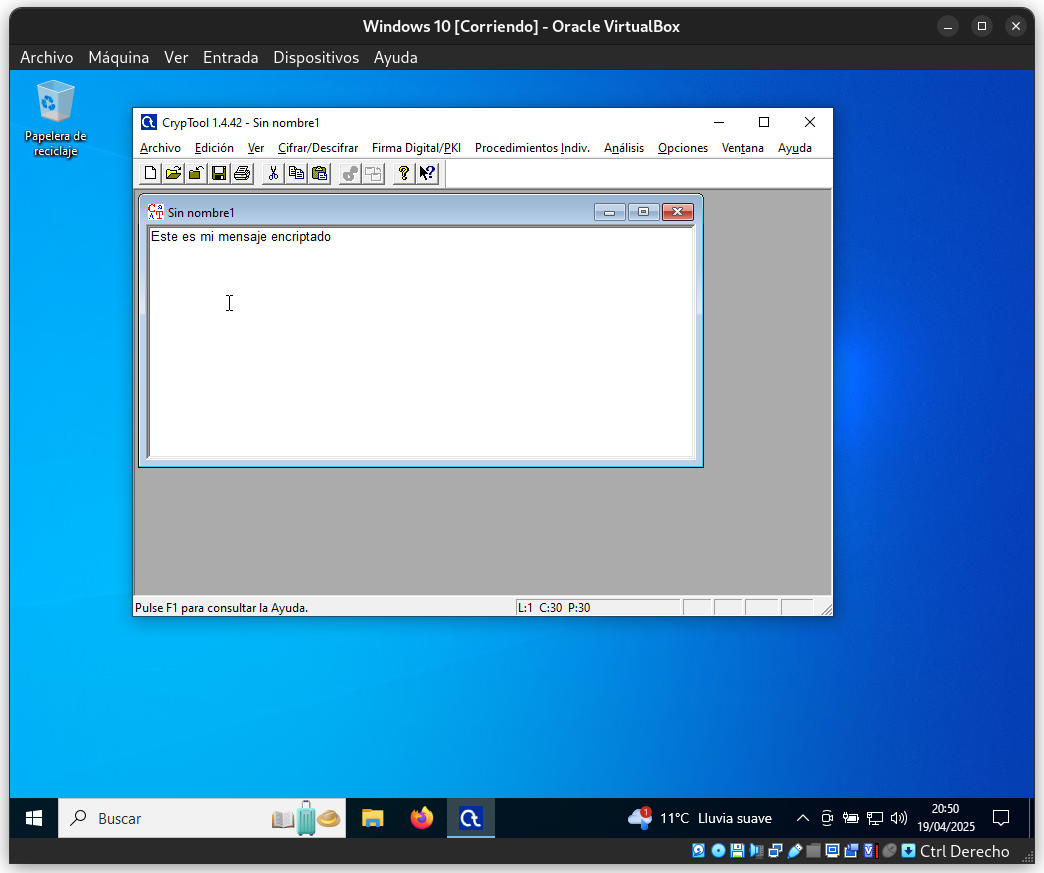
\includegraphics[width=\textwidth]{ClavesRSA-03.png}
    \caption{Pantalla del PIN de usuario}
\end{figure}

\begin{figure}[H]
    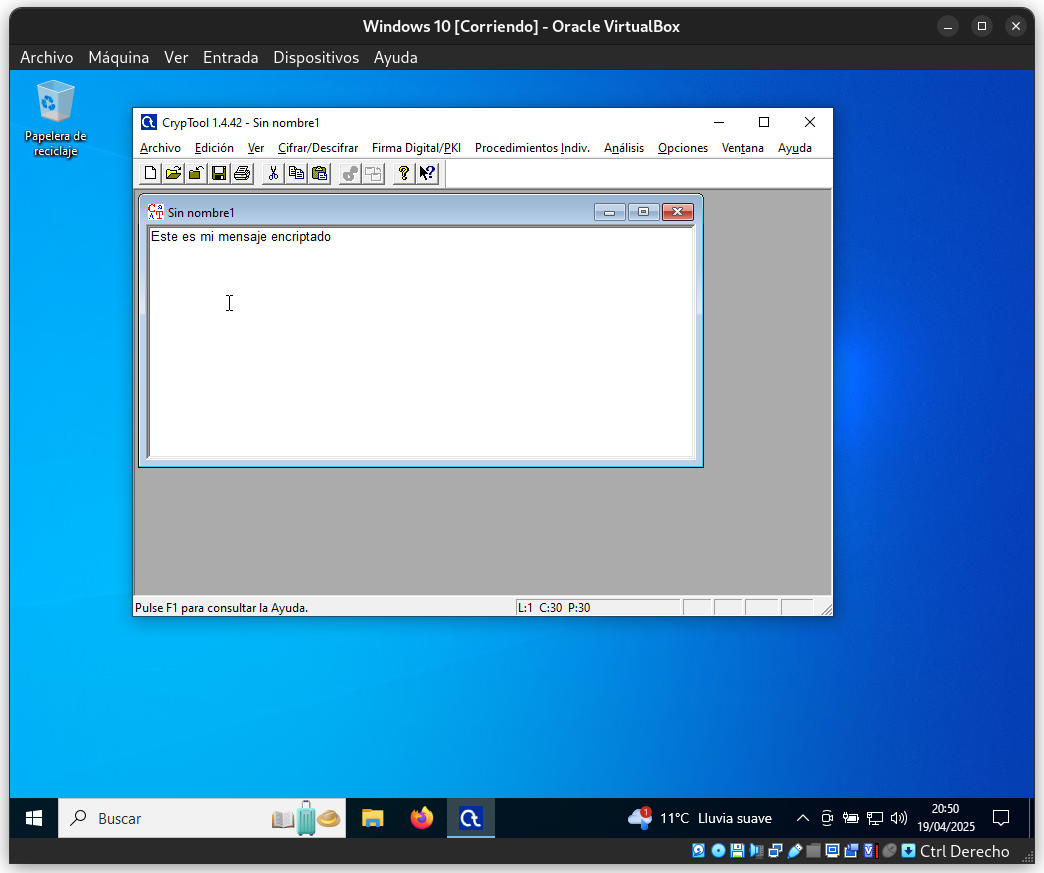
\includegraphics[width=\textwidth]{ClavesRSA-04.png}
    \caption{Texto de ejemplo para encriptar}
\end{figure}

\begin{figure}[H]
    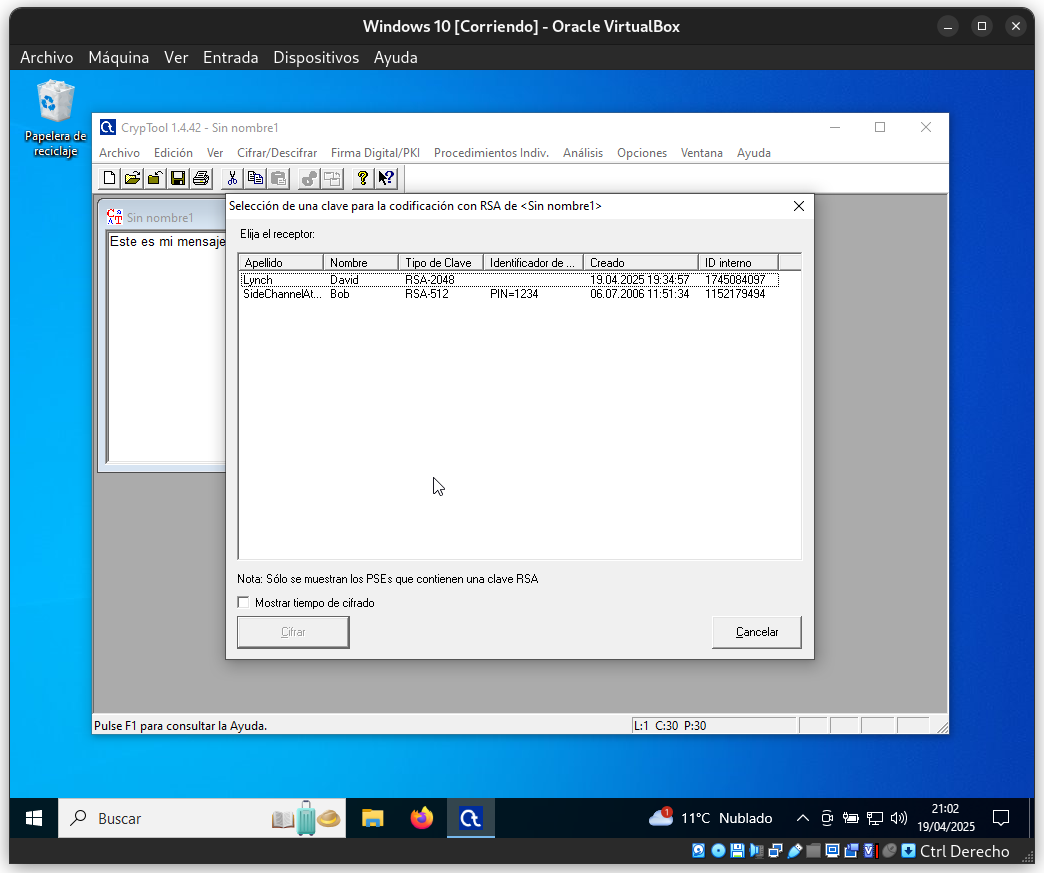
\includegraphics[width=\textwidth]{ClavesRSA-05.png}
    \caption{Generación del perfil del par de claves RSA}
\end{figure}

\begin{figure}[H]
    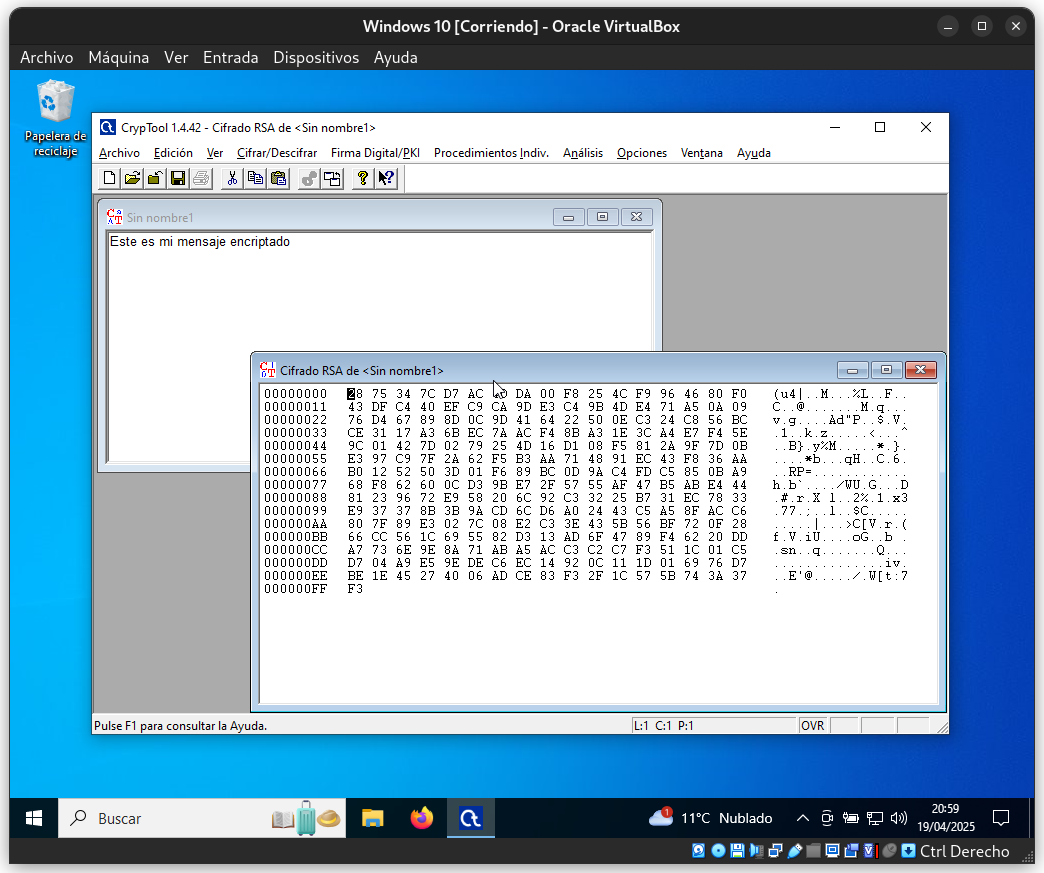
\includegraphics[width=\textwidth]{ClavesRSA-06.png}
    \caption{Generación del perfil del par de claves RSA}
\end{figure}

\begin{figure}[H]
    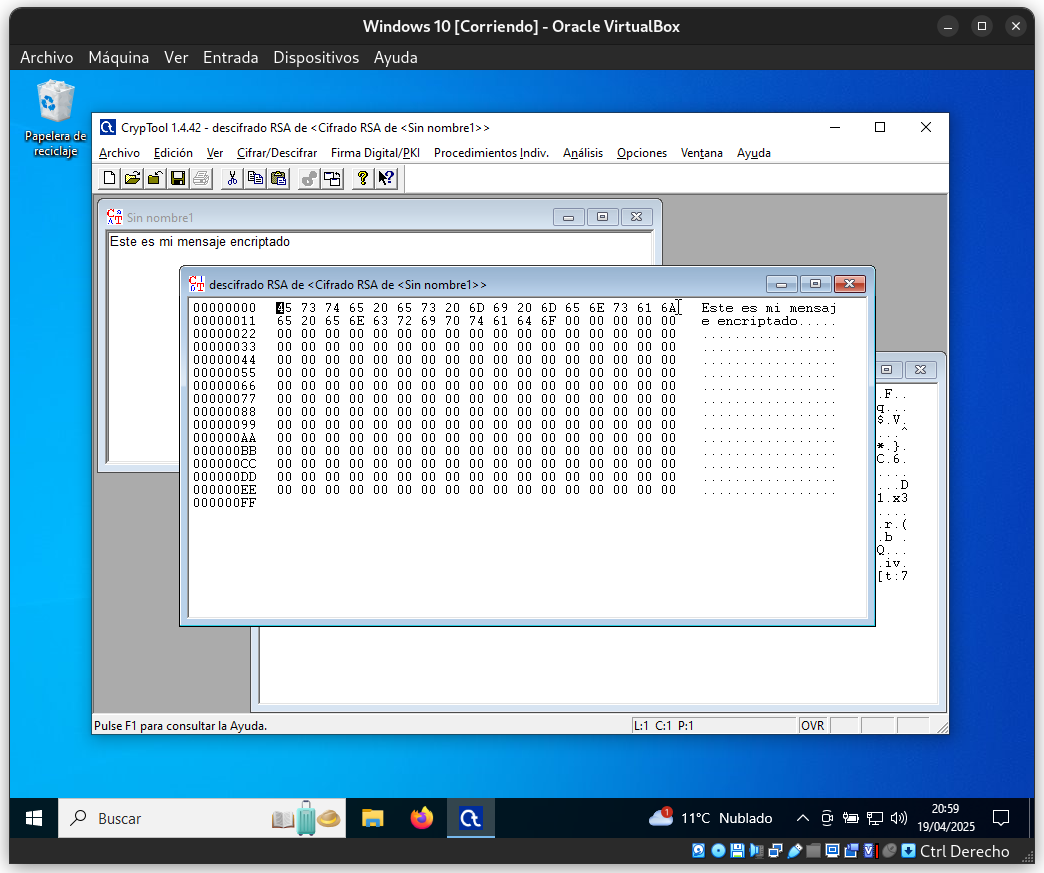
\includegraphics[width=\textwidth]{ClavesRSA-07.png}
    \caption{Generación del perfil del par de claves RSA}
\end{figure}


\subsubsection{¿Qué números conforman la clave pública?}

La clave pública está formada principalmente por dos números. El primero de ellos es el módulo ‘n’, que consiste en el producto de dos números primos (‘p’ y ‘q’ vistos en las clases teóricas) y es común tanto a la clave pública como a la privada. El segundo es el exponente público ‘e’, que suele tomar el valor de 65537. 

\subsubsection{¿A qué nos referimos con tamaño de clave?}

Como se explica en el apartado anterior, la clave está formada por dos números: ‘n’ y ‘e’. Que la clave tenga 2048 bits significa que el módulo ‘n’ tiene ese tamaño.  

Este tamaño nos indica la dificultad que tendría un ataque de fuerza bruta y el tamaño máximo a cifrar con esa clave. 


\subsubsection{Pruebas cifrado y descifrado}

\begin{figure}[H]
    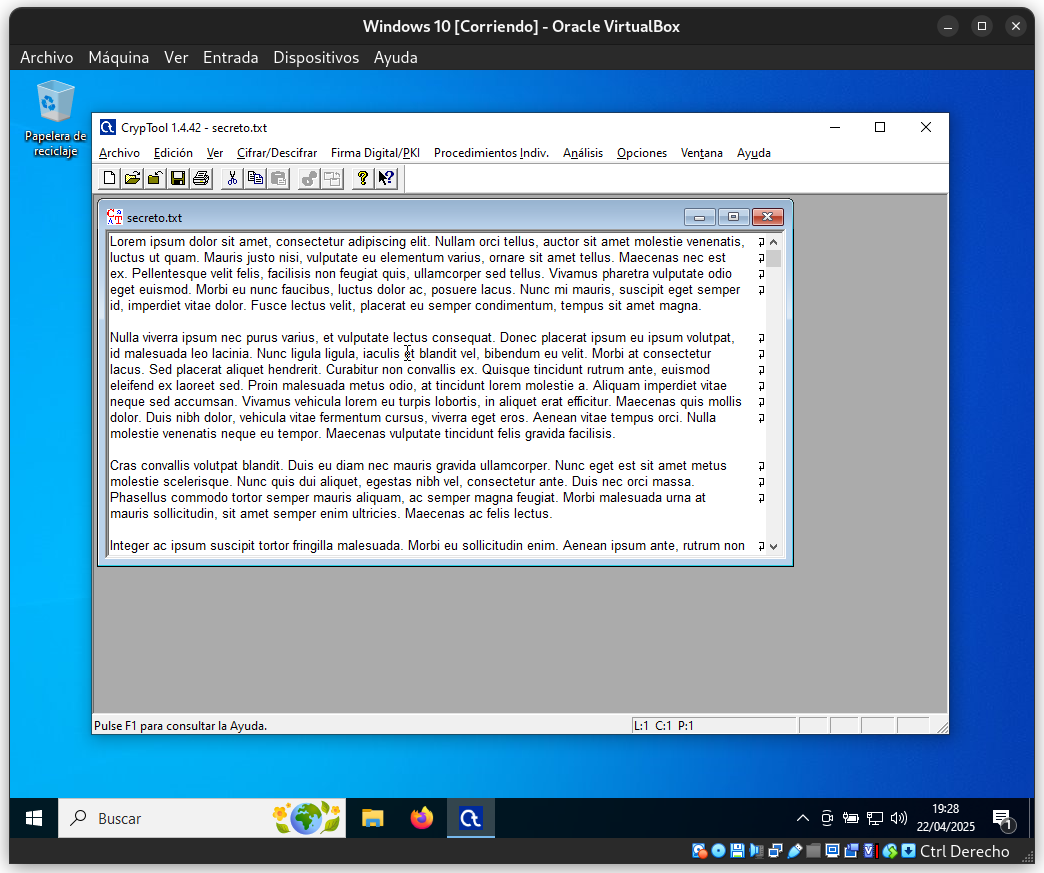
\includegraphics[width=\textwidth]{EncriptadoRSA-1}
    \caption{Generación del perfil del par de claves RSA}
\end{figure}

\begin{figure}[H]
    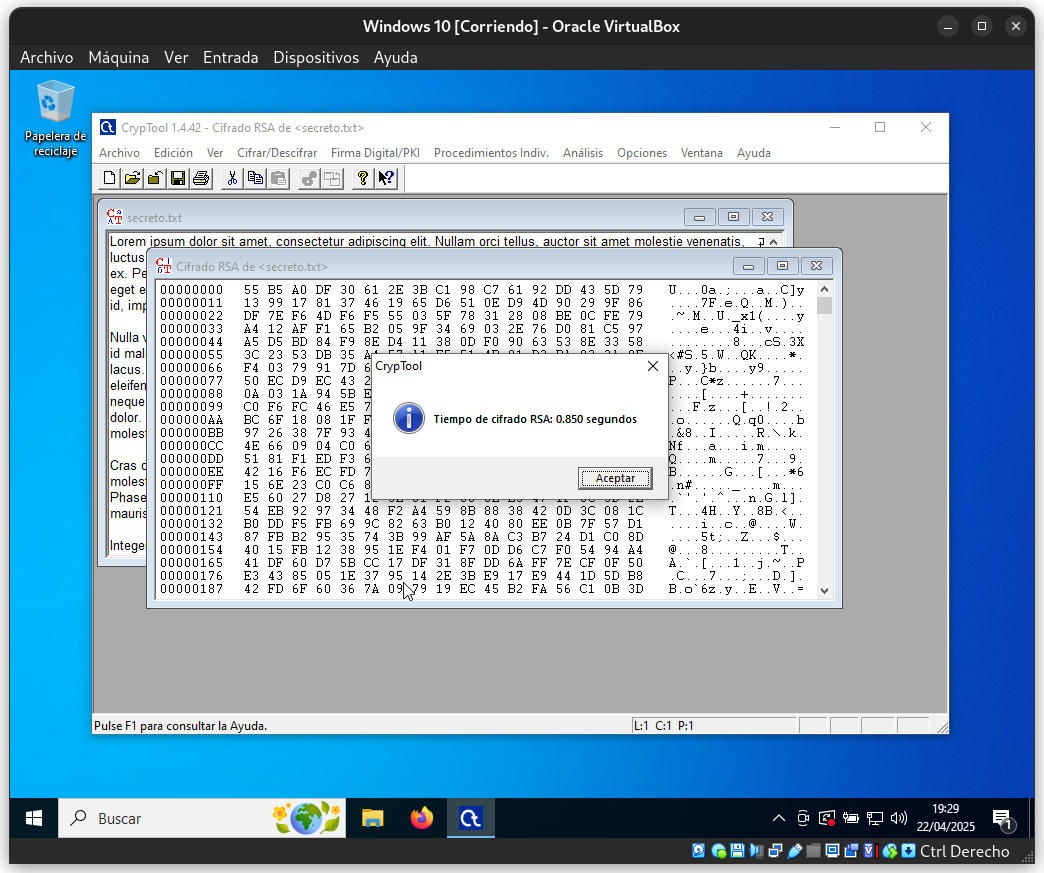
\includegraphics[width=\textwidth]{EncriptadoRSA-2}
    \caption{Generación del perfil del par de claves RSA}
\end{figure}

\begin{figure}[H]
    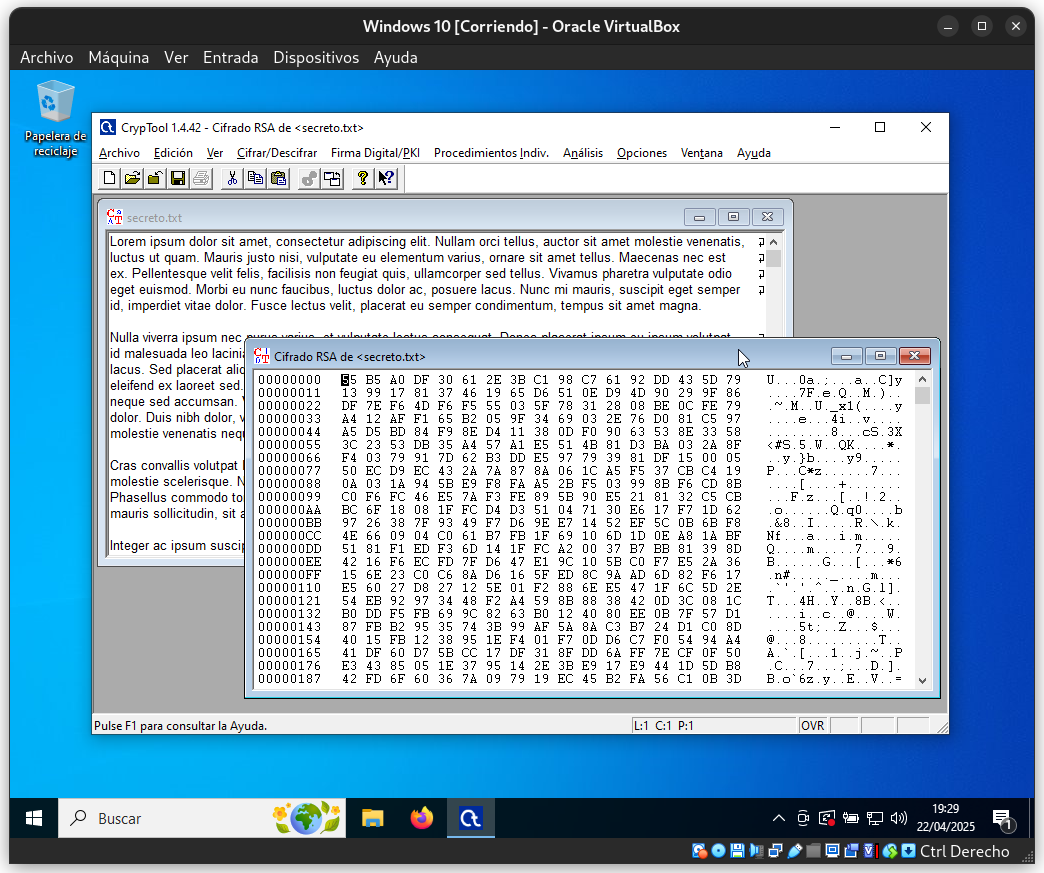
\includegraphics[width=\textwidth]{EncriptadoRSA-3}
    \caption{Generación del perfil del par de claves RSA}
\end{figure}

\begin{figure}[H]
    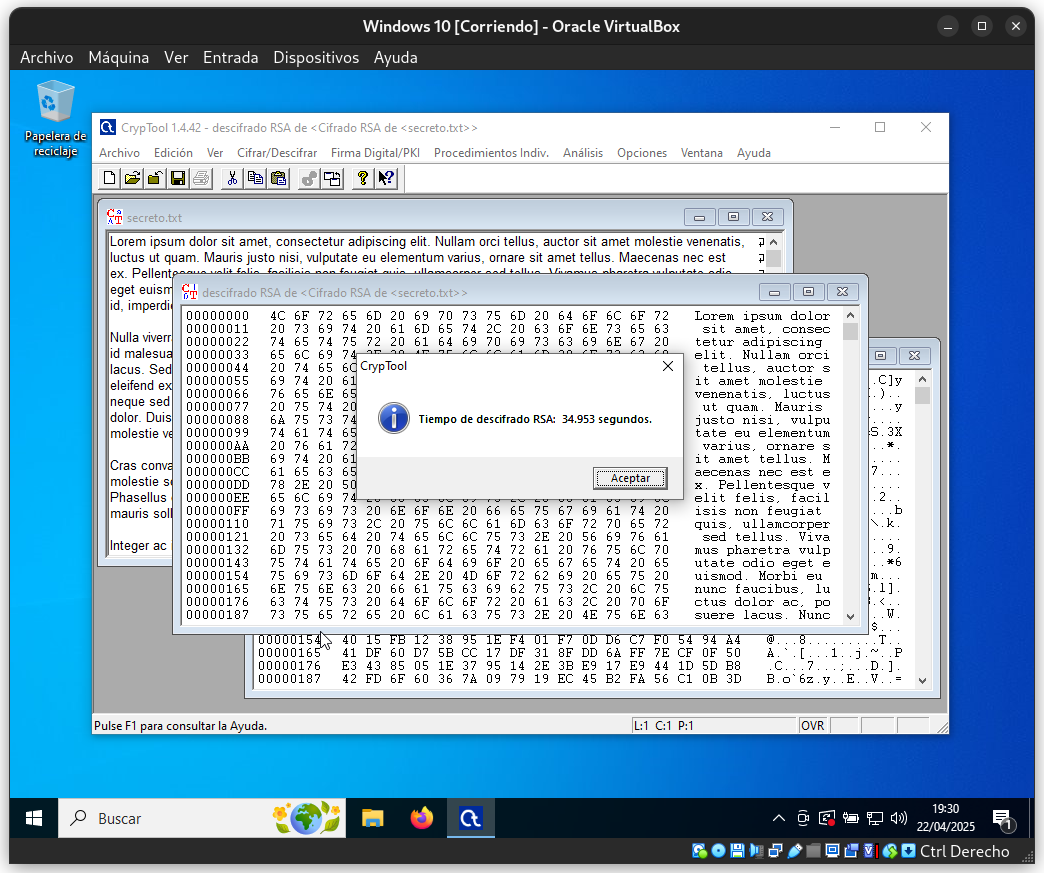
\includegraphics[width=\textwidth]{DesencriptadoRSA-1}
    \caption{Generación del perfil del par de claves RSA}
\end{figure}

\begin{figure}[H]
    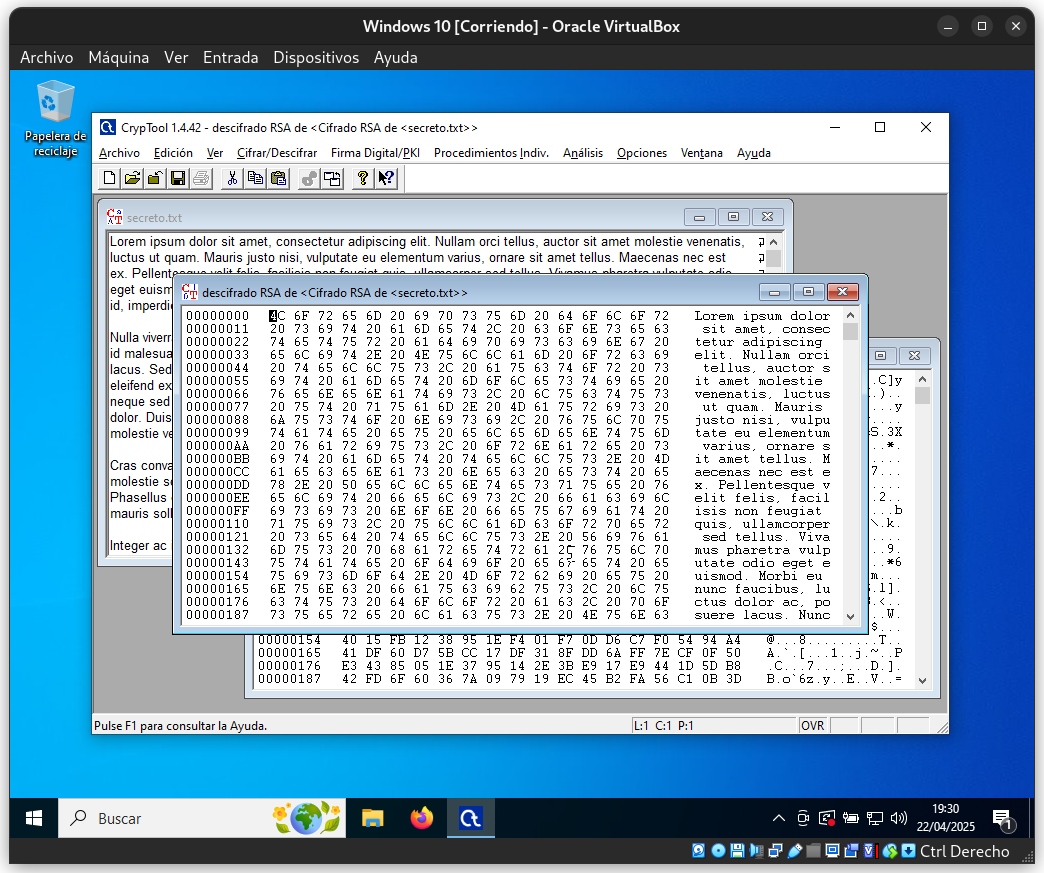
\includegraphics[width=\textwidth]{DesencriptadoRSA-2}
    \caption{Generación del perfil del par de claves RSA}
\end{figure}
